\chapter{Apache Kafka}
\label{intro-kafka}

As this thesis is about the implementation of a message broker that correlates
to the functionalities Apache Kafka provides, we describe in the following paragraphs the
components and functionalities of Apache Kafka in its current state (Version
0.8.2). This shall provide a basis for further comparison with
similar systems, which is why we won't provide any implementation-specific details in 
this section but describe the concepts in a higher level of
abstraction instead. Thus, it is also an overview and the initial position of our
own implementation. 

\section{Background}

Apache Kafka was initially developed at LinkedIn\cite{linkedin} and subsequently
released as an open source project with the Apache Software
Foundation\cite{apachefoundation}. 
\\ \\
Initially at LinkedIn the landscape was overwhelmed by the complexity due to
point-to-point (\ref{intro-messaging-pointtopoint})
pipelines that delivered data to a single destination with no
integration in between. Messages were written to aggregated files and then copied
to ETL servers (data integration) and further loaded into data warehousing and batch
processing (\ref{intro-datastream-batchprocessing})
clusters. Thus, this service suffered the lack of real-time data access which
is -- especially for a data driven company that populates activity-driven news
feeds -- an essential requirement. In fact, this fragility and complexity of this
pipeline lead to inevitable delays in adding new types of activity data.
Besides the feature-wise limitations, also the detection time of operational
problems increased over time due to the ever-increasing pressure on the latency
of the data warehouse processes. This could have been solved with
stream processing systems (\ref{intro-datastream-streamprocessing}) but was not
supported at this point, due to the lack of any central platform
(\ref{intro-datastream-centralplatform}) that can provide continuous data, .
\cite{goodhope2012building}

First attempts towards a piece of infrastructure (e.g. broker) that can server
stream and batch processing systems were made by experimenting with
ActiveMQ\cite{activemq}. During tests under full production load they ran into
several significant problems. It turned out that if the queue backed up beyond what could
be kept in memory, performance would be severely degraded due to heavy amounts of
random I/O. Inefficiencies had to be accepted regarding clustered consumers
requiring duplicating the data for each consumer in a separate queue. Further
difficulties were faced with ActiveMQ's built in persistence mechanism that lead
to very long restart times. 
\todo[inline]{well, reasons are not that overwhelming honestly...}
According to LinkedIn it would have been possible to provide enough buffer to
keep the ActiveMQ brokers above water but would have required hundreds of servers to
process a subset of activity data. As a result, the decision was made to build a
custom piece of messaging infrastructure targeting high-volume scale-out
deployment and thus serve batch and stream processing systems. 
\cite{goodhope2012building}

%TODO
\section{Use Cases}
\begin{description}
    \item [Traditional message broker]
    \item [Log aggregation]
    \item [Stream processing] Kafka's strong durability is very useful in the
        context of stream processing
\end{description}
\todo{incomplete}
\section{The Log}
\label{intro-kafka-log}
Apache Kafka uses a so-called commit log for managing messages within the
broker. This log has nothing in common with "application logging", as traces of
a software designed for human reading. Instead, logs in the context of distributed systems
are designed for programmatic access. Basically it is a simple, append-only data
structure which contains a sequence of records ordered by time where each
entry is assigned to a unique number called offset. Thanks to the strict
ordering inside a log the record offset can be used a timestamp where a log
gets decoupled from any time system. \cite{apachekafka} \cite{JK-TheLog}

\begin{figure}[H]
    \centering
    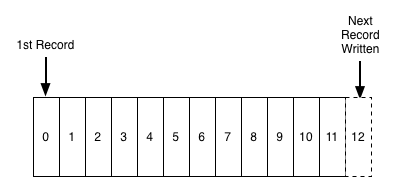
\includegraphics[width=0.4\textwidth]{images/log.png}
    \caption{The  Log \cite{JK-TheLog}}
    \label{fig:the-log}
\end{figure}

Apache Kafka handles its own log for every topic which contains all
published messages as single records. Compared to traditional messaging systems,
Kafka does not delete a record after consumption, actually it makes no difference
 whether or not they have been consumed. As we see later, every consumer
controls its position of the log on its own. Kafka can hold records within a
defined time window before it deletes the oldest records of the log.
Further more, an additional feature called log compaction can be activated to
reduce the amount of messages which need to be deleted by removing only obsolete
records. \cite{apachekafka} \cite{JK-TheLog}

Logs originate from from databases where they are used for replication and
recovery. Every change or update of a log leads to a new state that represents a
version including all the updates done in past. By describing every replica by the
latest log entry it has processed, the problem of coordinating states of
distributed replicas is getting much easier. Apache Kafka uses this approach for
consumption of messages. Every consumer knows its current offset and increases it
linearly as it reads messages from the log. The log can be seen as a re-playable
record of history whereas a consumer also can reset to an older state -- by using
the offset -- to reprocess. \cite{JK-TheLog}

\begin{figure}[H]
    \centering
    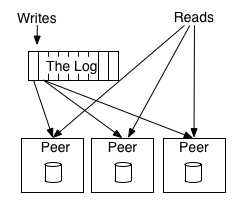
\includegraphics[width=0.4\textwidth]{images/state-machine-replication.png}
    \caption{Peers can sync their state with the log \cite{JK-TheLog}}
    \label{fig:the-log}
\end{figure}

\section{Components}

\subsection{Producer}

A producer can publish data to a topic of its choice and is responsible for
choosing which message will be assigned to which partition within a topic. In
fact, the producer sends data directly to the leader of a partition on the
broker. In order to help the producer find the correct server and partition
leader, Kafka can answer a request for meta-data about which servers are alive
and where the leaders for the partitions of a topic are at any given time. Thus
the producer can direct its requests appropriately. \cite{apachekafka}
\\ \\
The Kafka producer client can be configured to send messages in either a
synchronous or asynchronous fashion. The asynchronous mode allows the client to
batch (\ref{intro-kafka-components-batching}) small messages into larger data
chunks before sending them over the network. This can be configured to accumulate
no more than a fixed number of messages and to wait no longer than some fixed
latency bound (e.g. 64 kilobytes or 10 milliseconds). Thus, batching allows
fewer but larger I/O operations on the servers and results in higher throughput.
\cite{apachekafka} \cite{goodhope2012building}

\subsection{Consumer}
\label{subsec:kafka-consumer}

Apache Kafka introduces the concept of \textit{consumer groups} where consumers
label themselves with a consumer group name, and each message is delivered to
one consumer instance within each subscribing consumer group. Consumer groups
can be in separate processes or on separate machines.
\\ \\
In fact, this concept generalizes traditional queuing (\ref{intro-messaging-mom})
and publish-subscribe models (\ref{intro-messaging-publishsubscribe}).
If all consumer instances have the same consumer
group, then it works just like a traditional queue balancing over the consumers.
On the other hand, if all the consumer instances have different consumer groups,
it works like publish-subscribe.

\begin{figure}[H]
    \centering
    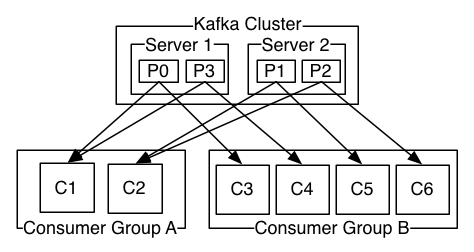
\includegraphics[width=0.6\textwidth]{images/consumer-groups.png}
    \caption{A two-server Kafka cluster hosting four partitions with two consumer groups. Consumer group A has two instances and group B has four \cite{apachekafka}}
    \label{fig:the-log}
\end{figure}

A consumer specifies its offset in the log within each request sent to the
broker and in return will receive back a chunk of log beginning from that
position. This leads to the fact that Kafka relies on the pull-model (as
described in \ref{intro-messaging-characteristics}) in order to reach a maximum
performance on the consumption side. As a side effect, the broker will be freed
from additional complexity regarding consumer handling from the broker. Another
advantage of Kafka relying on the pull-model results in the possibility of
aggressive batching of data sent to the consumer (see
\ref{intro-kafka-components-batching}). Apache Kafka avoids the naive approach
of busy-waiting for data to arrive but rather allows the consumer request to
block in a \gls{long poll}. \cite{apachekafka}
\\ \\
Unlike most other messaging systems, Apache Kafka does not keep track about what
messages have been consumed on the broker and thus does not rely on any
acknowledgements from the consumer. Instead, the position of a consumer is just
a single integer on a partition which defines the offset of the next message to
consume (see also \ref{intro-kafka-log}) for each specific consumer. As a side
benefit, a consumer can rewind back to an old offset and re-consume data. The
idea is to minimise the amount of state that Apache has to keep. Replicated state
is what makes fault-tolerance hard. \cite{apachekafka}


\subsection{Persistence}
\label{kafka-persistence}
Apache Kafka writes all data immediately to a persistent log
(\ref{intro-kafka-log}) 
and therefore relies heavily on the \gls{file system}.
Instead of flushing incoming messages from producers directly to the disks, the
data is stored as a compact byte structure within the \gls{page cache}.
\\ \\
The process of copying the data to the disk is handled by the operating system
that will not only use linear reads and writes \todo{gls} as a pattern for heavy
optimization but also provides read-ahead and write-behind techniques.
The latter will pre-fetch data in large block multiples and group smaller logical
writes into large physical writes. Thus, a SATA RAID-5 of six 7200rpm
disks will achieve a performance of 600MB/s in writes.
\\ \\
As a result of of the mentioned factors of using the file system and relying on
\gls{page cache} leads to the fact that Apache Kafka claims access to all free memory.
Doing so will result in a cache of up to 28-30GB on a 32GB machine. In a default
setup, data is kept in memory for 7 days to provide data required for processing
directly from the memory. This duration should be set according to one's own
needs. In fact, the memory stays persistent during a restart of the Kafka
service but won't if the server appliance reboots. Then the operating systems
flushes the memory. In the latter scenario, Apache Kafka will restore all data
from the hard disk to the memory.
\cite{apachekafka} \\ \\
One drawback following this model of not immediately writing data to disk can not be
omitted. A small number of messages can be lost in the event of a hard server
failure before messages are transfered to the Kafka brokers or flushed to disk.
\cite{goodhope2012building}

\subsection{Partitioning}
\label{kafka-partitioning}
Facing the challenges of large distributed systems, a log must scale well. For
improving scalability and fault tolerance, Kafka can divide a log in to multiple
partitions. This is a way to parallelize the consumption of the messages, whereas
the total number of partitions in a broker cluster needs to be at least the same
as the number of consumers (or producers) in a consumer (or producer) group.
Each partition is consumed by exactly one consumer (in a consumer group) and by
doing so, Kafka ensures that the consumer is the only reader of that partition
and consumes the data in order.

\begin{figure}[H]
    \centering
    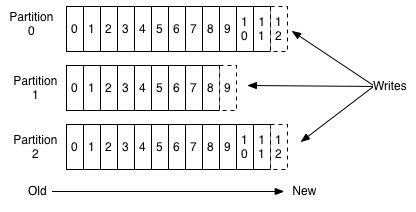
\includegraphics[width=0.5\textwidth]{images/log_anatomy.png}
    \caption{Partitioned Log \cite{apachekafka}}
    \label{fig:the-log}
\end{figure}

Each member -- be it on consumer or producer side -- will split the burden of
processing the topic between themselves according to the partitioning so that
one member will only be concerned with messages in the partition it is
assigned to. Thus, the throughput of the system will scale linearly with the
Kafka cluster size. \cite{apachekafka}


\subsection{Replication}
\label{kafka-replication}
To hold the defined guarantees (\ref{kafka-guarantees}) regarding to system
or network failures, Apache Kafka supports \gls{replication} on the level of log
partitions (\ref{kafka-partitioning}). Thereby it can replicate specific topics
across a configurable number of other Kafka servers (a.k.a. nodes). Every
topic has defined a leader node which is active in normal operation. Producers
send data directly to the leader broker. A leader node can have zero or
more followers which are responsible for replicating the entries of the active
log. The followers do this by simply acting as a normal Kafka consumer of the
leader node and constantly update their own log so that it is identical.
\cite{apachekafka}

If a leader node crashes, Kafka needs to choose a new one from among the
followers. Instead of using the common algorithm of quorum replication, it
has its own approach called in-sync replicas which is based on primary-backup
replication. In this algorithm the leader node
constantly keeps track of its followers by managing a set of \textit{in-sync}
nodes, called ISR (in-sync replicas). If one of these nodes crashes or falls
behind in replicating, the leader will dynamically remove it from its ISR. If a
follower comes back and catches up to the actual state the leader will reinsert
it. \textbf{Only members of this set can be elected as the new leader}. An incoming
message needs to be replicated by every \textit{in-sync} follower before any
other consumer can get it. A fully replicated message is considered as
\textit{committed}. This guarantees that the consumer need not worry about potentially
seeing a message that could be lost if the leader fails. \cite{apachekafka}
\cite{kafka-wiki-replication}

Apache Kafka always runs with Apache Zookeeper as the underlying manager for all
Kafka nodes. It handles the coordination between the leader and follower nodes
and also notifies producer and consumer about the presence or failure of brokers in a
Kafka system. The latter leads producers and consumers to coordinate their work
with different brokers. Regarding the replication of Kafka nodes, Zookeeper
also handles the leader election in case of failure. In order to do this, a leader node
constantly informs Zookeeper about changes in his ISR set. If the leader node
crashes, all surviving followers register themselves in Zookeeper. The replica that
registers first becomes the new leader. \cite{kafka-wiki-replication}
\cite{ArtKafkaInfoQ} \cite{apacheZookeeper}

\begin{figure}[H]
    \centering
    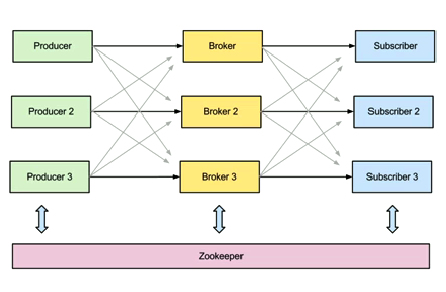
\includegraphics[width=0.55\textwidth]{images/kafka-replication-zookeeper.png}
    \caption{Zookeeper as underlying broker manager \cite{ArtKafkaInfoQ}}
    \label{fig:the-log}
\end{figure}

\subsection{Batching}
\label{intro-kafka-components-batching}

The trade-off between latency and throughput is addressed in Apache Kafka by
grouping small messages together -- referred to as batching. Rather than relying
on Nagle's algorithm on a TCP level, batching on the producer side is implemented
at the application level which allows precise timeout and message count
thresholds that trigger the sending. The broker itself does not do further batching
of file system writes but rather relies fully on the file system (as described in
\ref{kafka-persistence}) which brings an improvement so significant that it would
not make sense to further try to improve manually. Consumer data fetch requests
are also batched effectively by allowing the user to pull data from many
topics and partitions in a single request to avoid small requests on low-volume
topics. \cite{goodhope2012building}

\section{Guarantees}
\label{kafka-guarantees}
As a resume from the descriptions above we list guarantees of Kafka regarding
message delivery, fault tolerance and ordering. 

\begin{description}

\item[Delivery Model] \hfill \\
    Kafka guarantees at-least-once delivery by default and allows the user to
    implement at-most-once delivery by disabling retries on the producer and
    committing its offset prior to processing a batch of messages. Exactly-once
    delivery requires co-operation with the destination storage system but Kafka
    provides the offset which makes implementing this
    straight-forward.\cite{apachekafka}

\item[Fault Tolerance] \hfill \\
    It is guaranteed that any successfully published message will not be lost
    and can be consumed. Further more, a topic with replication
    (\ref{kafka-replication}) factor N will tolerate N-1 server failures without
    losing any messages. However there is no guarantee for the producer that
    a message is fully published in case of a network error. A feature which
    enables the producer to retry publishing a message as an idempotent
    request may be added in a later version of Kafka. \cite{apachekafka}

\item[Message Ordering] \hfill \\
    Thanks to the use of a log with sequential numbers for each entry (offset),
    Apache Kafka guarantees that messages from a producer to a topic partition
    will be appended in the order they are sent and consumers see messages
    in the order they are stored in the log. \cite{apachekafka}

\end{description}

%\section{Configuration Management (Zookeeper)}
%\subsection{PAXO Algorithm}
